\documentclass[border=2pt]{standalone}
\usepackage{mathptmx}\usepackage[scaled=0.92]{helvet}
\usepackage{xcolor}
\usepackage{tikz}
\usetikzlibrary{arrows.meta,positioning,fit,calc}
\usepackage{pgfplots}
\pgfplotsset{compat=1.17}
\definecolor{mapis}{RGB}{164,18,63}
\definecolor{slgray}{RGB}{138,148,156}
\begin{document}
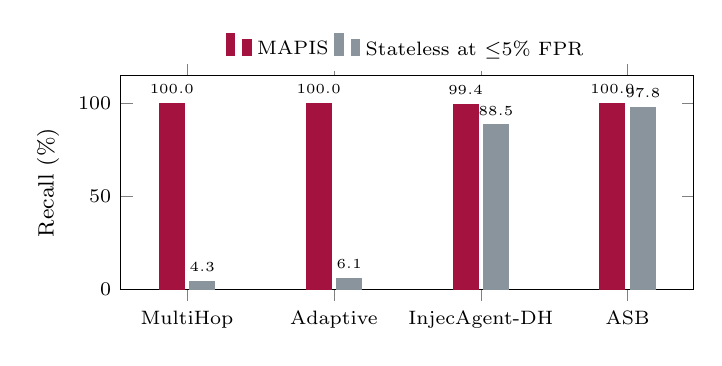
\begin{tikzpicture}
\begin{axis}[ybar, bar width=9pt, width=252pt, height=4.3cm, ymin=0, ymax=115, ylabel={Recall (\%)}, ylabel style={font=\footnotesize},
 symbolic x coords={MultiHop,Adaptive,InjecAgent-DH,ASB}, xtick=data, x tick label style={font=\scriptsize}, y tick label style={font=\scriptsize},
 legend style={at={(0.5,1.02)},anchor=south,legend columns=2,font=\scriptsize,draw=none}, nodes near coords={\pgfmathprintnumber[fixed,precision=1,fixed zerofill]{\pgfplotspointmeta}}, nodes near coords style={font=\tiny}, enlarge x limits=0.15]
\addplot[fill=mapis, draw=mapis] coordinates {(MultiHop,100) (Adaptive,100) (InjecAgent-DH,99.4) (ASB,100)};
\addplot[fill=slgray, draw=slgray] coordinates {(MultiHop,4.3) (Adaptive,6.1) (InjecAgent-DH,88.5) (ASB,97.8)};
\legend{MAPIS, Stateless at $\le$5\% FPR}
\end{axis}
\end{tikzpicture}
\end{document}
